% AeroCast Phase 1 report: IEEE conference skeleton.
% - Every result number comes from \input{generated/...}, produced by
%   scripts/make_report_tables.py from saved JSON artifacts. Do NOT type results by hand.
% - Prose drafted from the project documentation; the author must review and adapt it.
%   Red [TODO] markers remain only where information is genuinely missing (author block).
% - Compile with pdflatex + bibtex (e.g. on Overleaf, which provides IEEEtran.cls).
\documentclass[conference]{IEEEtran}
\IEEEoverridecommandlockouts
\usepackage{cite}
\usepackage{amsmath,amssymb}
\usepackage{graphicx}
\usepackage{booktabs}
\usepackage[table]{xcolor}
\usepackage{url}
\usepackage[hidelinks]{hyperref}
\graphicspath{{figures/}}

\newcommand{\todo}[1]{\textcolor{red}{[TODO: #1]}}
% Generated by scripts/make_report_tables.py from saved artifacts. Do not edit by hand.
%   audit: reports/audit/dataset_audit.json (sha256 0f79f814acf9)
%   design: reports/experiment/design_check.json (sha256 37409f892aaa)
%   features: reports/features/feature_validation.json (sha256 31b76bd33393)
%   stage7: reports/models/baseline_selection.json (sha256 955b2c61ad1e)
%   stage8: reports/calibration/stage8_results.json (sha256 02edcc5445c2)
%   test: reports/final/test_evaluation.json (sha256 bb4cab2e8df5)
%   stage9: reports/error_analysis/stage9_results.json (sha256 318a9bafb592)
\newcommand{\DataRows}{336,776}
\newcommand{\DataCols}{21}
\newcommand{\DataStart}{2013-01-01}
\newcommand{\DataEnd}{2013-12-31}
\newcommand{\DataLabelled}{327,346}
\newcommand{\DataUnlabelled}{9,430}
\newcommand{\DataNoDep}{8,255}
\newcommand{\DataDepNoArr}{458}
\newcommand{\DataArrNoDelay}{717}
\newcommand{\DataPositives}{80,100}
\newcommand{\DataPrevalence}{24.5\%}
\newcommand{\TrainRows}{217,727}
\newcommand{\TrainPos}{57,423}
\newcommand{\TrainPrev}{0.264}
\newcommand{\ValRows}{55,628}
\newcommand{\ValPos}{8,731}
\newcommand{\ValPrev}{0.157}
\newcommand{\TestRows}{53,991}
\newcommand{\TestPos}{13,946}
\newcommand{\TestPrev}{0.258}
\newcommand{\NFeatures}{31}
\newcommand{\NSchedFeatures}{13}
\newcommand{\NHistFeatures}{18}
\newcommand{\HistLag}{2}
\newcommand{\HistMinCount}{20}
\newcommand{\HistSmoothing}{20}
\newcommand{\MinPrecision}{70\%}
\newcommand{\TargetMinutes}{15}
\newcommand{\ValAPLR}{0.271}
\newcommand{\ValAPLRci}{0.271 [0.215, 0.318]}
\newcommand{\ValROCLR}{0.670}
\newcommand{\ValAPXGB}{0.235}
\newcommand{\ValROCXGB}{0.650}
\newcommand{\ValDiffAPci}{$-$0.036 [$-$0.056, $-$0.016]}
\newcommand{\DummyAccuracy}{84.3\%}
\newcommand{\CalSlopeA}{1.0096}
\newcommand{\CalInterceptB}{$-$0.4961}
\newcommand{\MaxPrecLR}{0.313}
\newcommand{\MaxPrecXGB}{0.377}
\newcommand{\CalSelLR}{sigmoid}
\newcommand{\CalSelXGB}{isotonic}
\newcommand{\TestAPLR}{0.363}
\newcommand{\TestAPLRci}{0.363 [0.311, 0.420]}
\newcommand{\TestROCLR}{0.626}
\newcommand{\TestROCLRci}{0.626 [0.599, 0.654]}
\newcommand{\TestBrierLR}{0.1904}
\newcommand{\TestLLLR}{0.5759}
\newcommand{\TestCITLLR}{$-$0.079}
\newcommand{\TestSlopeLR}{0.704}
\newcommand{\TestMeanPredLR}{0.179}
\newcommand{\TestAPXGB}{0.330}
\newcommand{\TestROCXGB}{0.609}
\newcommand{\TestBrierPrior}{0.1916}
\newcommand{\TestLLPrior}{0.5714}
\newcommand{\TestAPLift}{1.40}
\newcommand{\DiffAPLRXGB}{+0.033 [+0.018, +0.049]}
\newcommand{\DiffROCLRXGB}{+0.017 [+0.004, +0.030]}
\newcommand{\DiffAPLRPrior}{+0.104 [+0.079, +0.135]}
\newcommand{\DiffBrierLRPrior}{$-$0.0012 [$-$0.0068, +0.0063]}
\newcommand{\DiffLLLRPrior}{+0.0045 [$-$0.0154, +0.0311]}
\newcommand{\NovPrev}{0.181}
\newcommand{\DecPrev}{0.335}
\newcommand{\NovCITLLR}{$-$0.013}
\newcommand{\DecCITLLR}{$-$0.145}
\newcommand{\NovMeanPredLR}{0.168}
\newcommand{\DecMeanPredLR}{0.191}
\newcommand{\DecPriorShiftAdj}{0.372}
\newcommand{\DecPriorShift}{1.00}
\newcommand{\DecReqShift}{0.82}
\newcommand{\TestBootResamples}{200}
\newcommand{\TestBootUndefined}{0}


\begin{document}

\title{Flight Delay Prediction via Gradient Boosting and Temporal Deep Learning:\\
Phase~1 --- Leakage-Controlled Day-Ahead Machine-Learning Baselines}

\author{\IEEEauthorblockN{\todo{Author name(s)}}
\IEEEauthorblockA{\todo{Department, institution}\\
\todo{City, country}\\
\todo{email}}}

\maketitle

\begin{abstract}
We study whether a flight's arrival delay of at least \TargetMinutes{} minutes can be predicted
at the end of the day before departure, using only information available at that moment. On
\DataLabelled{} labelled departures from the three New York City airports in 2013, we define an
explicit prediction contract. Historical outcomes enter features only if their flight date is at
least \HistLag{} days earlier, a cutoff chosen because flights on the previous day can still be in
the air at prediction time. Logistic Regression and XGBoost are trained on January--August,
selected and calibrated on September--October, and evaluated once on November--December under a
frozen, pre-registered protocol with logged access to test labels. On the test period, the
calibrated Logistic Regression ranks flights better than chance and better than XGBoost: Average
Precision is \TestAPLR{} against a prevalence of \TestPrev{}, and ROC AUC is \TestROCLR{}. Its
probabilities, however, are no more accurate than a constant base-rate forecast, and they
under-predict in December, when the delay rate rose sharply. No decision threshold reached the
targeted \MinPrecision{} precision on validation, so no operating point was frozen. The results
indicate what a strictly day-ahead model can offer: modest, honest risk ranking, not reliable
individual delay alarms.
\end{abstract}

\begin{IEEEkeywords}
flight delay prediction, gradient boosting, logistic regression, probability calibration,
temporal validation, data leakage
\end{IEEEkeywords}

% =====================================================================
\section{Introduction}\label{sec:intro}
Flight delays impose costs on passengers, airlines and airports. A day-ahead estimate of delay
risk could support passenger information and planning. However, much of the published delay
prediction work operates close to departure, using live airspace or surveillance information that
is not available a day in advance~\cite{rebollo2014,gui2020}. Results obtained under different
prediction horizons are therefore not directly comparable. A model evaluated with information it
would not have had at prediction time can also look far better than it is. This is the problem of
leakage~\cite{kaufman2012}.

This report addresses a deliberately strict question: \emph{using only information available at
the end of the previous day, can a classifier predict whether a flight will arrive at least
\TargetMinutes{} minutes late, and how reliable are its probabilities on later, unseen months?}
The contributions are:
\begin{itemize}
\item an explicit prediction contract, including a historical-outcome cutoff chosen from evidence
about when outcomes become known;
\item leakage-controlled features whose temporal correctness is verified by independent tests;
\item a chronological train/validation/test design with a single, pre-registered test evaluation
and logged access to test labels;
\item an analysis of ranking quality, probability quality and calibration over time, with
baselines and day-level uncertainty intervals;
\item honest reporting of negative findings: no operating point at the targeted precision, and
calibration deterioration under seasonal shift.
\end{itemize}
Temporal deep-learning models belong to Phase~2 of the project and are outside the scope of this
report.

\subsection{Problem formulation}
For flight $i$ with scheduled date $D_i$, the label is
\begin{equation}
y_i = \mathbb{1}\!\left[\text{arr\_delay}_i \geq \TargetMinutes\ \text{min}\right],
\end{equation}
following the BTS on-time convention~\cite{bts_ontime}. The model outputs
$\hat{p}_i = \Pr(y_i = 1 \mid \mathbf{x}_i)$, where $\mathbf{x}_i$ may contain only information
available at the end of day $D_i - 1$. Flights without a recorded arrival delay are excluded and
never labelled. For cancelled or diverted flights the arrival delay is undefined. Labelling them
on time would be wrong, and labelling them delayed would change the meaning of the target. The
model's population is therefore flights that operated and have a recorded arrival delay
(Section~\ref{sec:data}).

% =====================================================================
\section{Related Work}\label{sec:related}
\textbf{Surveys.} Carvalho et al.~\cite{carvalho2021} review data-science approaches to flight
delays. They propose a taxonomy organised by problem scope, data and computational method, and
trace research trends in the field.

\textbf{Short-horizon prediction with live system state.} Rebollo and
Balakrishnan~\cite{rebollo2014} predict departure delays 2--24~h ahead with random forests. Their
features include network-wide variables describing the delay state of the US National Airspace
System at prediction time. Gui et al.~\cite{gui2020} combine ADS-B surveillance messages with
weather, schedule and airport information. They report overfitting for an LSTM on their dataset and
a random forest reaching 90.2\% binary accuracy. Kim et al.~\cite{kim2016} model day-to-day
sequences of airport delays with deep LSTM networks. These designs rely on information that exists
only close to departure, which a day-ahead model cannot use.

\textbf{Longer horizons.} Choi et al.~\cite{choi2016} train decision trees, random forests,
AdaBoost and $k$-nearest neighbours on US domestic flight and weather data. At prediction time they
use the flight schedule and weather \emph{forecasts}, address class imbalance by resampling, and
compare models by accuracy and ROC curves. According to the summary in~\cite{zoutendijk2021}, they
consider horizons of one and five days. Lambelho et al.~\cite{lambelho2020} use machine-learning
predictions of delays and cancellations to assess strategic schedules at London Heathrow, where
slots are allocated months ahead.

\textbf{Costs and probabilities.} Choi et al.~\cite{choi2017} make classifiers cost-sensitive by
subsampling according to misclassification costs, and evaluate a weighted error whose optimum
depends on the cost ratio between false positives and false negatives. Zoutendijk and
Mitici~\cite{zoutendijk2021} predict full delay distributions for individual flights at a Dutch
airport. They use mixture density networks and random-forest regression, evaluate with the
continuous ranked probability score (a proper scoring rule), and construct train and test sets by
5-fold cross-validation. They argue that most prior work reports classes or point estimates,
which convey no uncertainty.

\textbf{Gap.} In the reviewed literature, horizons and the information assumed available at
prediction time vary widely and are often implicit. Headline results are frequently accuracy or
confusion-matrix metrics~\cite{choi2016,kim2016,gui2020}, which can mislead under class
imbalance~\cite{saito2015}. Probabilistic quality is rarely assessed, and validation designs are
often not chronological~\cite{zoutendijk2021}. None of the reviewed studies combines an explicit
day-ahead information contract with a verified historical-outcome cutoff; a single, pre-registered
chronological test evaluation; imbalance-aware ranking metrics together with proper scoring rules
and calibration assessed over time; and explicit reporting of negative operational results. This
work does not claim higher accuracy than prior studies. It positions itself as a leakage-controlled
baseline that shows what a strictly day-ahead model can and cannot deliver. The review is small and
non-systematic, so this gap refers to the reviewed sample, not the whole field.

% =====================================================================
\section{Data and Quality Assessment}\label{sec:data}
The supplied file matches the public \texttt{nycflights13} dataset~\cite{nycflights13}, sourced
from BTS on-time data: \DataRows{} scheduled departures from EWR, JFK and LGA between \DataStart{}
and \DataEnd{} (Table~\ref{tab:dataset}).
A scripted audit checked the file before any modelling:
\begin{itemize}
\item there are no duplicate rows, and every calendar day of the year is present;
\item clock fields are valid, and recorded departure and arrival delays reconcile exactly with the
difference between actual and scheduled times (allowing for flights that cross midnight);
\item the rows are \emph{not} in chronological order (months appear in lexicographic order), so
all processing sorts by reconstructed timestamps and never relies on row position;
\item there are no cancellation, diversion, delay-cause, weather or time-zone fields. Because the
scheduled departure is in New York local time and the scheduled arrival in destination local time,
a true scheduled duration cannot be computed, so distance is used instead.
\end{itemize}
Cancellation and diversion are inferred from missing fields. A flight with no departure time never
departed (\DataNoDep{} flights); \DataDepNoArr{} departed but have no arrival time; and
\DataArrNoDelay{} arrived but have no recorded delay. These \DataUnlabelled{} flights are excluded
from the modelling population. Their share differs across carriers and months, so the exclusion is
not random. The model therefore describes delay \emph{conditional on the flight operating and being
recorded}. Among the \DataLabelled{} labelled flights, \DataPositives{} (\DataPrevalence) arrived at
least \TargetMinutes{} minutes late. The scope is limited to departures from the three New York
airports in a single year.
% Generated from reports/audit/dataset_audit.json, reports/features/feature_validation.json. Do not edit by hand.
\begin{table}[!t]
\centering
\footnotesize
\caption{Dataset summary (supplied file; NYC departures, 2013).}
\label{tab:dataset}
\begin{tabular}{lr}
\toprule
Quantity & Value \\
\midrule
Rows $\times$ columns & 336,776 $\times$ 21 \\
Date range & 2013-01-01 to 2013-12-31 \\
Labelled flights (arrival delay recorded) & 327,346 \\
Delayed ($\geq$15 min) / prevalence & 80,100 / 24.5\% \\
Excluded: never departed (cancellation proxy) & 8,255 \\
Excluded: departed, no arrival time & 458 \\
Excluded: arrived, no delay recorded (diversion proxy) & 717 \\
Features (schedule / historical) & 31 (13 / 18) \\
\bottomrule
\end{tabular}
\end{table}


% =====================================================================
\section{Prediction Contract and Leakage Prevention}\label{sec:contract}
Leakage is the use of information about the target that would not legitimately be available when
the prediction is made~\cite{kaufman2012}. To prevent it, every flight scheduled on date $D$ is
scored at a fixed time: the end of day $D-1$, i.e.\ 00:00 local time on $D$. A field may describe
the flight being predicted only if it is known from the published schedule at that time:
\begin{itemize}
\item \textbf{Permitted:} scheduled departure and arrival times, date, carrier, origin,
destination and distance.
\item \textbf{Prohibited:} actual departure and arrival times, departure delay, arrival delay
(which defines the target) and airborne time, all of which are observed only on day $D$.
\item \textbf{Excluded as unverifiable:} the aircraft tail number. Assignments change on the day
(same-day swaps are visible in the data), so its value at the end of $D-1$ cannot be established.
\end{itemize}
The rules are enforced in code by a field registry: feature definitions must declare their source
columns, and any non-permitted column is rejected.

Outcomes of \emph{other, earlier} flights may enter historical features, but only if they were
already known at prediction time. A cutoff based on flight date alone ($< D$) is not enough. A
lower bound on a flight's landing time is its actual departure time plus its airborne time, both
recorded in the data. Some flights dated $D-1$, disproportionately the delayed ones, provably land
after midnight, so their outcomes were unknown at the end of $D-1$. Including them would leak
target-correlated information. With the cutoff at flight dates $\leq D-\HistLag$, no flight violated
this, even when three hours were added for unrecorded taxiing. The \HistLag-day lag was therefore
adopted.

% =====================================================================
\section{Exploratory Data Analysis}\label{sec:eda}
To avoid informing design choices with later outcomes, all analyses relating the target to
candidate features used the training period only. Full-year views were restricted to label-free
quantities and per-period delay rates. The main findings, each tied to a design decision, are:
\begin{itemize}
\item \textbf{Time of day.} The delay share rises steadily from early-morning to evening departures
(Fig.~\ref{fig:hour}), so departure and arrival hour enter as features.
\item \textbf{Calendar.} Weekdays differ (Saturday has the lowest delay share). Monthly
differences exist, but training covers only January--August, so month values in the validation
and test periods would be unseen. Month is therefore excluded, and seasonal level enters only
through lagged historical rates.
\item \textbf{Airports and routes.} Delay shares for many destinations and routes lie outside the
range expected from sampling noise alone. Many routes, however, have few flights. This motivates
shrunk historical route rates instead of a one-hot route identity.
\item \textbf{Seasonality.} The validation months are the calmest period of the year, while the
test period includes a volatile December (Fig.~\ref{fig:daily}). This warns that thresholds and
calibration chosen on validation may transfer poorly.
\item \textbf{Schedule mix.} The carrier, airport and departure-hour composition changes little
between periods. The main temporal change is in the outcome rate itself.
\end{itemize}
The full-year monthly delay rates, including those of the test months, were seen during the data
audit before the split was fixed. This is disclosed in Section~\ref{sec:limitations}.
\begin{figure}[!t]
\centering
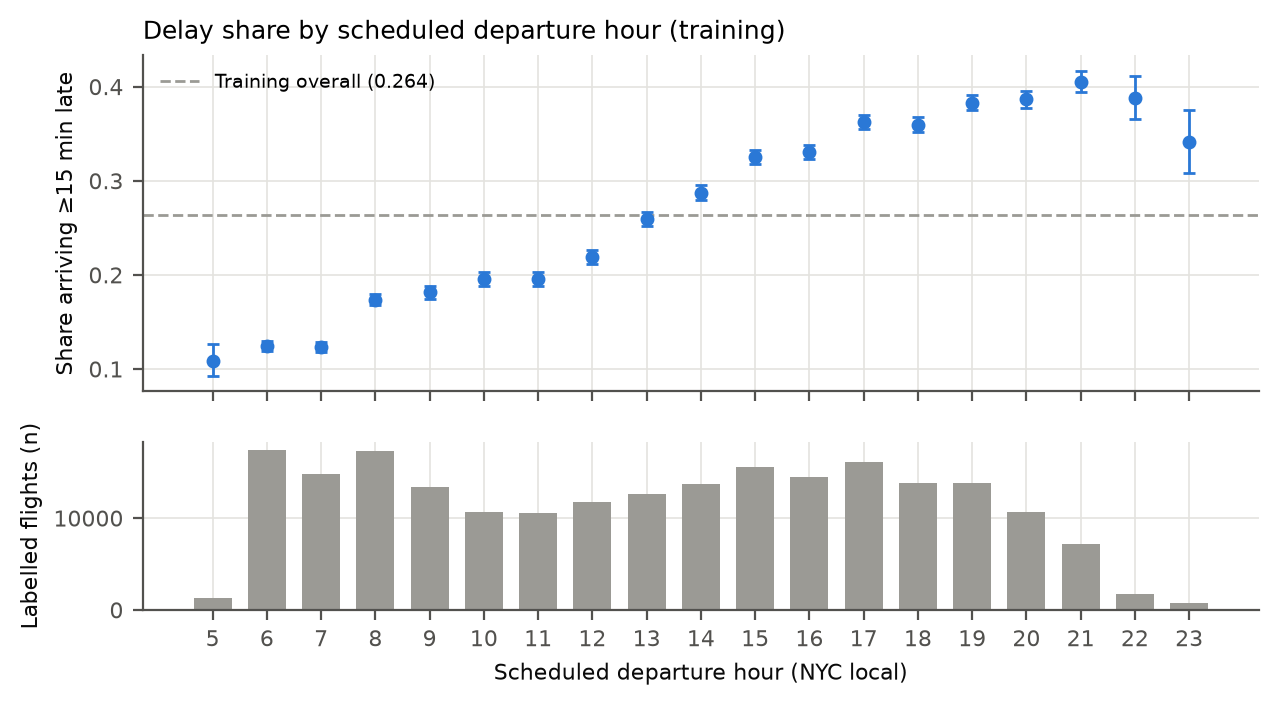
\includegraphics[width=\linewidth]{eda_dep_hour.png}
\caption{Training-period delay share by scheduled departure hour, with Wilson 95\% intervals and
sample sizes.}
\label{fig:hour}
\end{figure}
\begin{figure*}[!t]
\centering
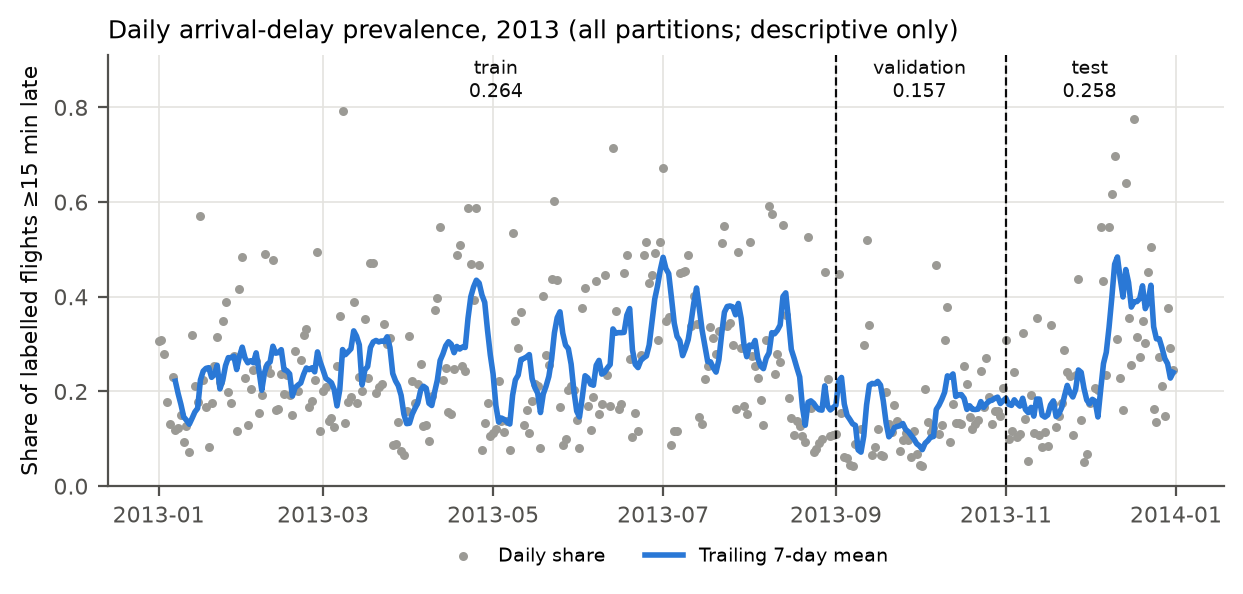
\includegraphics[width=0.85\linewidth]{eda_daily_prevalence.png}
\caption{Daily delay prevalence in 2013 with partition boundaries (descriptive).}
\label{fig:daily}
\end{figure*}

% =====================================================================
\section{Feature Engineering}\label{sec:features}
The model uses \NFeatures{} features: \NSchedFeatures{} schedule features and \NHistFeatures{}
historical features. Time of day is encoded cyclically,
\begin{equation}
h_{\sin} = \sin\!\left(\tfrac{2\pi h}{24}\right), \qquad h_{\cos} = \cos\!\left(\tfrac{2\pi h}{24}\right).
\end{equation}
Historical delay rates for an entity $e$ (carrier, origin, destination, route) over a window ending
at $D-\HistLag$ are shrunk towards the system-wide rate $\pi$ of the same window:
\begin{equation}
\tilde{r}_e =
\begin{cases}
\dfrac{k_e + m\,\pi}{n_e + m}, & n_e \geq n_{\min},\\[4pt]
\pi, & n_e < n_{\min},
\end{cases}
\end{equation}
with $k_e$ delayed flights out of $n_e$ labelled flights, $m=\HistSmoothing$ and $n_{\min}=\HistMinCount$.
Shrinkage pulls the rate of a sparsely observed entity towards the system-wide rate, so a route
with a handful of flights is not treated as a stable risk estimate. The fallback applies
when an entity has too little history. Rates are computed over an expanding window and a 28-day
window, and system-wide rates also over a 7-day window. Counts of labelled flights are included for
the fixed windows only. Expanding-window counts grow monotonically with the date, so they act as a
hidden time index whose test values lie entirely outside the training range; they were removed.

Each historical feature is computed from per-day outcome totals and cumulative sums. Its value for
date $D$ therefore depends only on flights dated $\leq D-\HistLag$. By construction it cannot
include the flight's own outcome, same-day outcomes or later records. This is verified by tests
that:
\begin{itemize}
\item recompute the features of randomly sampled flights independently, by direct filtering;
\item check that changing every outcome on one date leaves all features before date $+\HistLag$
unchanged;
\item check that appending future records, or removing all test-period rows, does not change
earlier features;
\item check that shuffling the input rows has no effect.
\end{itemize}
Flights on the first \HistLag{} days of the year have no eligible history. Their historical
features are left missing rather than filled from later data.

% =====================================================================
\section{Experimental Design}\label{sec:design}
Partitions are chronological (Table~\ref{tab:protocol}). Validation is used for model selection
(Average Precision), XGBoost early stopping, calibration choice and the threshold rule. The test
set was evaluated once, under a frozen, hash-bound manifest with logged label access.
A deployed model is trained on the past and applied to the future. A chronological holdout
reproduces this ordering, whereas a random split would let models learn from flights that occur
after the ones they are evaluated on. That matters here for two reasons. First, the process is
non-stationary: the delay rate changes strongly with the season (Fig.~\ref{fig:daily}), and a
random split would hide this shift by mixing all seasons into both sides. Second, historical
features summarise earlier outcomes, so evaluation must follow the same ordering they were built
for. Bergmeir and Ben\'{\i}tez~\cite{bergmeir2012} note that temporal dependence violates the
assumptions of cross-validation in theory, but they found no practical harm in their experiments
and recommend \emph{blocked} cross-validation. Their work therefore does not, by itself, rule out
random splits. Our choice rests on non-stationarity and deployment realism.

The split uses whole calendar months, so no day is divided between partitions. All models are
fitted on the training months only and are \emph{not} refitted on training plus validation. The
calibrator and threshold are estimated on predictions for data the model has not seen, and a refit
would produce a different model whose calibration was never checked. The cost is that the
validation months do not contribute to fitting. Because validation is reused for selection, early
stopping and calibration, validation scores are optimistic development estimates. The test period
gives the single reported estimate.
% Generated from reports/experiment/design_check.json, reports/final/test_evaluation.json, configs/config.yaml. Do not edit by hand.
\begin{table*}[!t]
\centering
\footnotesize
\caption{Experimental protocol and chronological partitions.}
\label{tab:protocol}
\begin{tabular}{lcrrr}
\toprule
Partition & Dates & Labelled & Delayed & Prevalence \\
\midrule
Train & 2013-01-01 to 2013-08-31 & 217,727 & 57,423 & 0.264 \\
Validation & 2013-09-01 to 2013-10-31 & 55,628 & 8,731 & 0.157 \\
Test (single evaluation) & 2013-11-01 to 2013-12-31 & 53,991 & 13,946 & 0.258 \\
\bottomrule
\end{tabular}
\par\vspace{2pt}\parbox{\linewidth}{\scriptsize Prediction at the end of day $D-1$; historical outcomes only from flight dates $\leq D-2$. Target: arrival delay $\geq$ 15 min. Threshold rule: maximise recall subject to precision $\geq$ 70\% on validation (infeasible; see Sec.~\ref{sec:calibration}).}
\end{table*}


% =====================================================================
\section{Models}\label{sec:models}
\subsection{Logistic Regression}
With $\hat{p}_i = \sigma(\beta_0 + \boldsymbol{\beta}^{\top}\mathbf{x}_i)$ and
$\sigma(z) = 1/(1+e^{-z})$, the model is linear in the log-odds. Training minimises
\begin{equation}
\tfrac{1}{2}\lVert\boldsymbol{\beta}\rVert_2^2
- C\sum_{i}\big[y_i\log\hat{p}_i + (1-y_i)\log(1-\hat{p}_i)\big],
\end{equation}
where $\boldsymbol{\beta}$ are the coefficients, $\beta_0$ the intercept (not penalised),
$\mathbf{x}_i$ the preprocessed features of flight $i$, and $C>0$ the inverse regularisation
strength~\cite{hastie2009}. The second term is $C$ times the binary cross-entropy (log loss): it
rewards high predicted probability for the observed outcome. The first term, the $L_2$ penalty,
shrinks coefficients towards zero. Smaller $C$ means stronger shrinkage, trading a little bias for
lower variance, which helps when the relationship between features and delays drifts over time. A
coefficient $\beta_j$ is the change in the log-odds of delay per unit change in feature $j$ (a
standardised unit for numeric inputs), holding the others fixed. This is an association, not a
causal effect.

The search covered $C\in\{0.01,0.1,1,10\}$, with and without balanced class weights. The selected
model ($C=0.01$, unweighted, lbfgs solver) uses the strongest regularisation in the grid; validation
AP varied little across the grid. Preprocessing is fitted on training rows only:
\begin{itemize}
\item time of day is encoded cyclically and numeric features are standardised;
\item historical counts are log-transformed;
\item carrier, origin and destination are one-hot encoded, with categories seen in fewer than 100
training flights grouped into an ``infrequent'' column, to which unseen categories are also
mapped;
\item missing historical rates (the first days of the year) are imputed with training medians, and
a missing-history indicator lets the model treat these rows differently.
\end{itemize}

\subsection{Gradient-boosted trees (XGBoost)}
XGBoost~\cite{chen2016} builds an additive model $F(\mathbf{x}) = \sum_{k=1}^{K} \eta f_k(\mathbf{x})$
of regression trees~\cite{friedman2001}, with $\hat{p} = \sigma(F)$, by minimising
\begin{equation}
\sum_{i}\ell\big(y_i, F(\mathbf{x}_i)\big) + \sum_{k}\Big(\gamma T_k + \tfrac{\lambda}{2}\lVert\mathbf{w}_k\rVert^2\Big).
\end{equation}
Here $f_k$ is the $k$-th regression tree, $\eta$ the learning rate (shrinkage), $\ell$ the
logistic loss on the log-odds $F$, $T_k$ the number of leaves of tree $k$, $\mathbf{w}_k$ its leaf
weights, and $\gamma,\lambda\geq 0$ penalties on tree size and leaf weights. Trees are added one at
a time. Each new tree is fitted using a second-order approximation of the loss around the current
model, with gradients $g_i=\partial\ell/\partial F=\hat{p}_i-y_i$ and curvatures
$h_i=\partial^2\ell/\partial F^2=\hat{p}_i(1-\hat{p}_i)$. For a fixed tree structure, the optimal
weight of leaf $j$ is
\begin{equation}
w_j^{*} = -\frac{G_j}{H_j + \lambda}, \qquad G_j = \sum_{i \in j} g_i,\quad H_j = \sum_{i \in j} h_i ,
\end{equation}
so $\lambda$ shrinks leaf predictions, much as the $L_2$ penalty does in Logistic Regression. The
sparsity-aware split finding of XGBoost sends missing values along a learned default direction,
so the missing historical features of the first days need no imputation~\cite{chen2016}.
Tree ensembles remain strong baselines on tabular data~\cite{grinsztajn2022}.

The search varied tree depth $\{3,5,7\}$, minimum child weight $\{1,20\}$ and the positive-class
weight (none, or the training negative-to-positive ratio). The fixed settings were $\eta=0.05$,
row and column subsampling of 0.8, and the library defaults $\lambda=1$, $\gamma=0$. The number of
trees was set by early stopping on validation Average Precision. The selected model (depth 3,
minimum child weight 20, class-weighted) stopped after only a small number of trees. Deeper models
fit the training months much better but validated worse, suggesting patterns that did not carry
over to the autumn. Class weighting barely changed validation AP but distorted the raw
probabilities upwards, which the calibration step later corrects.

\subsection{Reference baselines}
Two trivial references anchor the comparison. The \emph{most-frequent dummy} always predicts ``not
delayed'' ($\hat{p}=0$). It would be \DummyAccuracy{} accurate on validation while detecting no
delays at all, which is why accuracy is not used as a headline metric. The \emph{prior baseline}
always predicts the training delay rate (\TrainPrev{}). It has no ranking ability, but it is the
natural reference for probability quality: a useful model should beat it on Brier score and log
loss.

% =====================================================================
\section{Evaluation Metrics and Calibration}\label{sec:calibration}
\subsection{Ranking metrics}
Let $q_i\in[0,1]$ be the predicted delay probability of flight $i$, $y_i\in\{0,1\}$ its label, and
$N$ the number of flights. Flagging every flight with $q_i\geq t$ gives, at threshold $t$,
\begin{equation}
P(t) = \frac{\mathrm{TP}(t)}{\mathrm{TP}(t)+\mathrm{FP}(t)},\qquad
R(t) = \frac{\mathrm{TP}(t)}{\mathrm{TP}(t)+\mathrm{FN}(t)},
\end{equation}
where TP, FP and FN count true positives, false positives and false negatives. Precision $P$ is the
share of flagged flights that are actually delayed; recall $R$ is the share of delayed flights that
are flagged. Average Precision summarises the precision--recall curve without choosing a threshold:
\begin{equation}
\mathrm{AP}=\sum_{n}\big(R_n-R_{n-1}\big)\,P_n ,
\end{equation}
where $(P_n, R_n)$ are the precision and recall at the $n$-th distinct threshold, in decreasing
order of $t$. A random or constant predictor has AP equal to the prevalence, so AP is judged
against the base rate. ROC AUC is the probability that a randomly chosen delayed flight receives a
higher score than a randomly chosen on-time flight; random ranking gives 0.5. Under class imbalance,
ROC plots can give an overly favourable impression, while precision--recall analysis reflects the
reliability of positive predictions~\cite{saito2015,davis2006}. AP is therefore the primary
selection metric, with ROC AUC secondary.

\subsection{Probability quality}
The Brier score~\cite{brier1950} and the log loss are
\begin{equation}
\mathrm{BS}=\frac{1}{N}\sum_{i}(q_i-y_i)^2,\qquad
\mathrm{LL}=-\frac{1}{N}\sum_{i}\big[y_i\log q_i+(1-y_i)\log(1-q_i)\big].
\end{equation}
Both are strictly proper scoring rules: their expected value is minimised only by reporting the true
probability~\cite{gneiting2007}. They reward calibration and sharpness together. Log loss penalises
confident errors heavily (probabilities are clipped to $[10^{-15},1-10^{-15}]$).

\subsection{Calibration}
A model is calibrated if, among flights predicted with probability $q$, a fraction $q$ are actually
delayed: $\Pr(y=1\mid \hat{q}=q)=q$. Ranking quality does not imply this. Boosted trees are known to
distort probabilities~\cite{niculescumizil2005}, and poorly calibrated predictions can mislead
decisions even when ranking is good~\cite{guo2017,vancalster2019}. Raw model outputs $p$ are mapped
to calibrated probabilities $q$ by one of two methods.
\begin{itemize}
\item \textbf{Sigmoid (Platt) scaling}~\cite{platt2000}: $q=\sigma\big(a\,\mathrm{logit}(p)+b\big)$,
with $\mathrm{logit}(p)=\log\frac{p}{1-p}$ and $(a,b)$ fitted by logistic regression. This
two-parameter monotone map can correct a shifted or overly spread score scale.
\item \textbf{Isotonic regression}~\cite{zadrozny2002}: $q=g(p)$, where $g$ is the non-decreasing
step function minimising $\sum_i(y_i-g(p_i))^2$. It is more flexible but needs more data.
\end{itemize}
Both are compared with no calibration by cross-fitting within validation. Each method is fitted on
September and scored by log loss on October, and then the reverse. The method with the lowest mean
held-out log loss is selected; within $10^{-6}$, the simpler method wins. The selected method is
then refitted on all validation predictions. The rule selected \CalSelLR{} scaling for Logistic
Regression ($a=\CalSlopeA$, $b=\CalInterceptB$) and \CalSelXGB{} regression for XGBoost
(Table~\ref{tab:calibration}). The slope $a\approx 1$ means the ranking spread of Logistic
Regression transferred to the validation months, and the calibration mainly corrected the
probability level downwards for the calmer autumn.
% Generated from reports/calibration/stage8_results.json. Do not edit by hand.
\begin{table}[!t]
\centering
\footnotesize
\caption{Calibration choice by Sep$\leftrightarrow$Oct cross-fitting (mean held-out values on validation).}
\label{tab:calibration}
\begin{tabular}{llcc}
\toprule
Model & Method & Log loss & Brier \\
\midrule
LR & none & 0.4279 & 0.1316 \\
LR & sigmoid (selected) & 0.4139 & 0.1267 \\
LR & isotonic & 0.4185 & 0.1274 \\
XGBoost & none & 0.6688 & 0.2384 \\
XGBoost & sigmoid & 0.4183 & 0.1280 \\
XGBoost & isotonic (selected) & 0.4178 & 0.1278 \\
\bottomrule
\end{tabular}
\par\vspace{2pt}\parbox{\linewidth}{\scriptsize No threshold reached 70\% precision on calibrator-unseen validation predictions (maximum precision: LR 0.313, XGBoost 0.377).}
\end{table}


\subsection{Operating threshold}
The operational requirement was a minimum precision of $\pi_{\min}=$\MinPrecision{}. The threshold
is selected on validation as
\begin{equation}
t^{*}=\arg\max_{t}\; R(t)\quad\text{subject to}\quad P(t)\geq \pi_{\min},
\end{equation}
with ties resolved towards the highest threshold. The predictions used are ones the calibrator did
not see: raw probabilities if no calibration is selected, otherwise cross-fitted ones (September
calibrated by the October fit, and vice versa). No threshold satisfied the constraint. The highest
attainable precision was \MaxPrecLR{} for Logistic Regression and \MaxPrecXGB{} for XGBoost, so
the requirement was declared infeasible and \emph{no operating threshold was frozen}. The
requirement was not relaxed. One limitation of the procedure is that the two monthly calibration
maps shift the months differently, which reorders some flights between months and slightly lowers
pooled ranking quality. On raw scores, the target precision is reached only by a handful of the
highest-ranked validation flights, and only in some bootstrap resamples, so the conclusion is
unchanged.

\subsection{Uncertainty: day-level bootstrap}
Flights on the same day share weather and congestion, so they are not independent. Intervals are
therefore computed by resampling whole flight dates. Let $d_1,\dots,d_K$ be the $K$ dates of an
evaluation period. A bootstrap sample draws $K$ dates with replacement and pools all their flights,
and the metric is recomputed on it. Over $B=$\TestBootResamples{} samples, the 2.5th and 97.5th
percentiles of the recomputed metric form the 95\% interval. Resampling whole clusters keeps the
within-day dependence~\cite{field2007}. For a paired difference between two models, both are
evaluated on the same resampled dates. The interval assumes that days are exchangeable within a
period, an approximation under seasonality.

% =====================================================================
\section{Results}\label{sec:results}
\subsection{Validation (development)}
% Generated from reports/models/baseline_selection.json. Do not edit by hand.
\begin{table*}[!t]
\centering
\footnotesize
\caption{Validation comparison (development estimate; optimistic because validation was used for selection).}
\label{tab:validation}
\begin{tabular}{lcccc}
\toprule
Model & AP [95\% CI] & ROC AUC [95\% CI] & Brier & Log loss \\
\midrule
Most-frequent dummy & 0.157 [0.133, 0.178] & 0.500 & 0.1570 & 5.421 \\
Prior (train prevalence) & 0.157 [0.133, 0.178] & 0.500 & 0.1437 & 0.467 \\
Logistic Regression & 0.271 [0.215, 0.318] & 0.670 [0.641, 0.696] & 0.1318 & 0.428 \\
XGBoost & 0.235 [0.187, 0.279] & 0.650 [0.624, 0.676] & 0.2385 & 0.669 \\
\bottomrule
\end{tabular}
\par\vspace{2pt}\parbox{\linewidth}{\scriptsize Day-block bootstrap, 200 resamples. Raw (uncalibrated) probabilities.}
\end{table*}

Table~\ref{tab:validation} reports development results on September--October (prevalence
\ValPrev{}). They are optimistic, because the same months were used to select configurations and
to stop XGBoost early. Logistic Regression reached a validation AP of \ValAPLRci{} and ROC AUC
\ValROCLR{}. XGBoost reached an AP of \ValAPXGB{} and ROC AUC \ValROCXGB{}. The paired difference
(XGBoost $-$ Logistic Regression) in AP was \ValDiffAPci{}, an interval excluding zero. Following
the pre-registered rule (highest validation AP), Logistic Regression was carried forward as the
primary model, with XGBoost as the comparison.

\subsection{Single frozen test evaluation}
% Generated from reports/final/test_evaluation.json. Do not edit by hand.
\begin{table*}[!t]
\centering
\footnotesize
\caption{Single pre-registered test evaluation (Nov--Dec 2013).}
\label{tab:test}
\begin{tabular}{lcccccc}
\toprule
Model & AP & ROC AUC & Brier & Log loss & CITL & Slope \\
\midrule
LR + sigmoid (primary) & 0.363 [0.311, 0.420] & 0.626 [0.599, 0.654] & 0.190 [0.169, 0.216] & 0.576 [0.522, 0.642] & $-$0.079 & 0.704 \\
XGBoost + isotonic & 0.330 [0.279, 0.386] & 0.609 [0.586, 0.634] & 0.195 [0.172, 0.221] & 0.587 [0.531, 0.654] & $-$0.089 & 0.660 \\
Prior baseline & 0.258 [0.222, 0.302] & 0.500 [0.500, 0.500] & 0.192 [0.175, 0.212] & 0.571 [0.534, 0.616] & 0.005 & undefined \\
Most-frequent dummy & 0.258 [0.222, 0.302] & 0.500 [0.500, 0.500] & 0.258 [0.222, 0.302] & 8.921 [7.679, 10.417] & $-$0.258 & undefined \\
\bottomrule
\end{tabular}
\par\vspace{2pt}\parbox{\linewidth}{\scriptsize 95\% day-block bootstrap intervals (200 resamples; undefined resamples across all intervals: 0). CITL: mean predicted minus observed rate. Threshold-dependent metrics not applicable: no operating threshold was frozen (D32).}
\end{table*}

% Generated from reports/final/test_evaluation.json. Do not edit by hand.
\begin{table*}[!t]
\centering
\footnotesize
\caption{Paired test differences (same resampled days).}
\label{tab:paired}
\begin{tabular}{lcccc}
\toprule
Comparison & $\Delta$AP & $\Delta$ROC & $\Delta$Brier & $\Delta$Log loss \\
\midrule
LR $-$ XGBoost & +0.033 [+0.018, +0.049] & +0.017 [+0.004, +0.030] & $-$0.0042 [$-$0.0064, $-$0.0022] & $-$0.0113 [$-$0.0189, $-$0.0047] \\
LR $-$ prior & +0.104 [+0.079, +0.135] & +0.126 [+0.099, +0.154] & $-$0.0012 [$-$0.0068, +0.0063] & +0.0045 [$-$0.0154, +0.0311] \\
\bottomrule
\end{tabular}
\par\vspace{2pt}\parbox{\linewidth}{\scriptsize AP/ROC $>0$ and Brier/log loss $<0$ favour the primary model.}
\end{table*}

The test period (\TestRows{} labelled flights, prevalence \TestPrev{}) was evaluated once with all
decisions frozen (Tables~\ref{tab:test} and~\ref{tab:paired}). These are the reported results.
\begin{itemize}
\item \textbf{Ranking.} The calibrated Logistic Regression achieved an AP of \TestAPLRci{}, which is
\TestAPLift{} times the prevalence, and a ROC AUC of \TestROCLRci{}. It outperformed XGBoost
(AP difference \DiffAPLRXGB{}; ROC AUC difference \DiffROCLRXGB{}) and the prior baseline in AP
(\DiffAPLRPrior{}). Discrimination was lower than on validation.
\item \textbf{Probability quality.} The model was \emph{not} better than the constant prior. The
Brier difference was \DiffBrierLRPrior{} and the log-loss difference \DiffLLLRPrior{}; both
intervals include zero, and the log-loss point estimate is slightly worse.
\item \textbf{Calibration.} The model under-predicted delays: mean predicted probability
\TestMeanPredLR{} against an observed rate of \TestPrev{}, a calibration-in-the-large of
\TestCITLLR{}. The calibration slope of \TestSlopeLR{} (ideal~1) indicates predictions that are
too spread out on the test data (Fig.~\ref{fig:test}).
\item \textbf{Operating point.} No operating threshold --- the \MinPrecision{} precision target was
infeasible on validation. Recall at the target precision, precision, recall, F1 and the confusion
matrix at an operating threshold are therefore not reported. The descriptive test precision--recall
curve also stays below the target precision.
\end{itemize}
None of the bootstrap resamples produced an undefined metric (\TestBootUndefined{} undefined
resamples).
\begin{figure*}[!t]
\centering
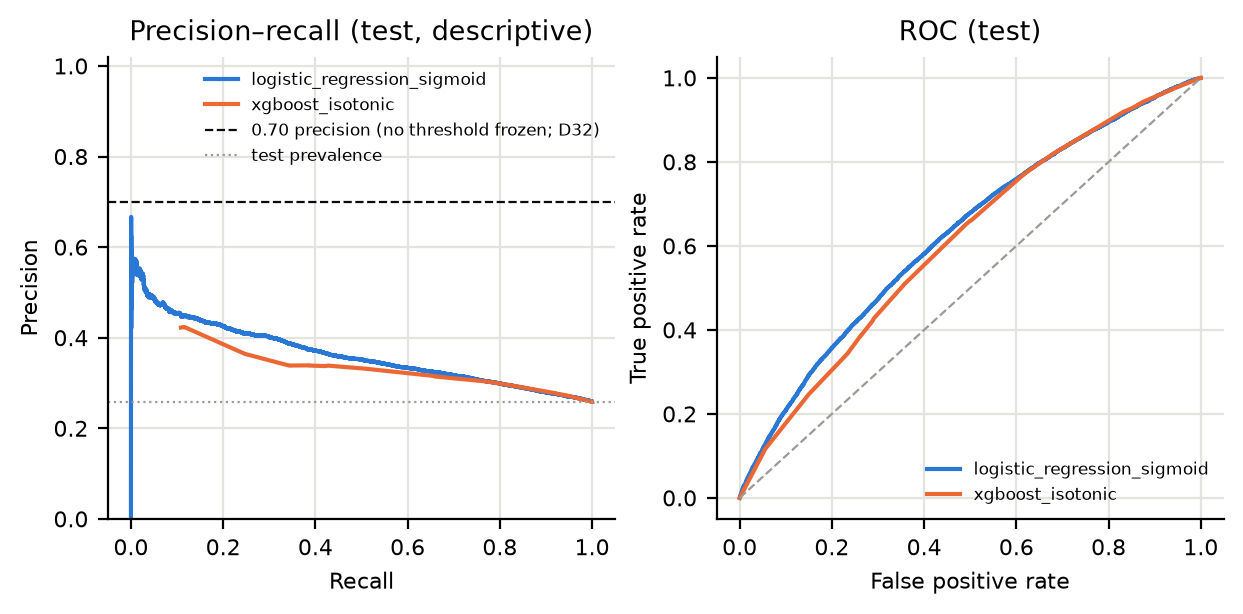
\includegraphics[width=0.48\linewidth]{test_pr_roc.png}\hfill
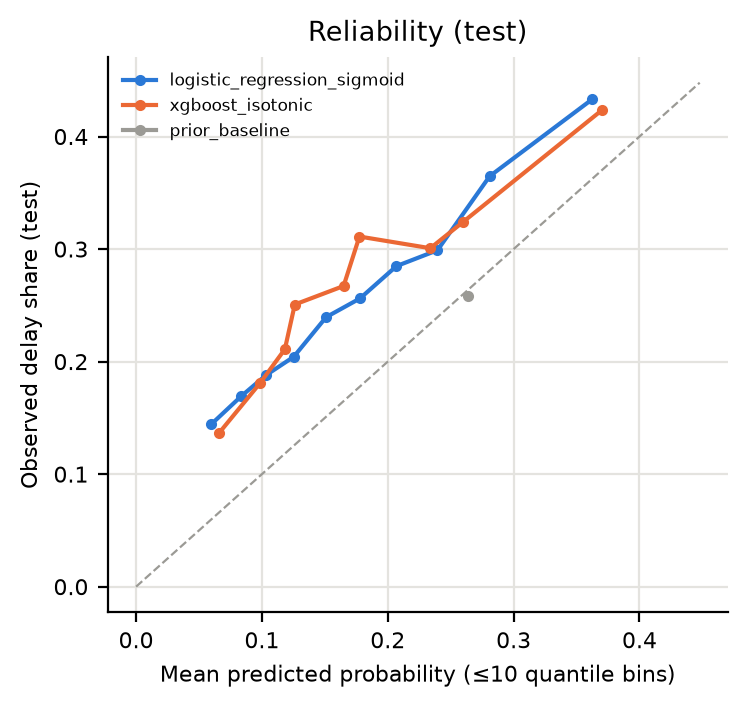
\includegraphics[width=0.30\linewidth]{test_reliability.png}
\caption{Test precision--recall and ROC curves (descriptive; no threshold read from them) and
test reliability diagram.}
\label{fig:test}
\end{figure*}

% =====================================================================
\section{Error Analysis}\label{sec:error}
% Generated from reports/final/test_evaluation.json. Do not edit by hand.
\begin{table*}[!t]
\centering
\footnotesize
\caption{Test results by month (descriptive).}
\label{tab:monthly}
\begin{tabular}{llcccccc}
\toprule
Month & Model & Prev. & Mean pred. & CITL & AP & ROC & Brier \\
\midrule
2013-11 & LR + sigmoid & 0.181 & 0.168 & $-$0.013 & 0.274 & 0.634 & 0.1435 \\
2013-11 & Prior & 0.181 & 0.264 & 0.083 & 0.181 & 0.500 & 0.1551 \\
2013-12 & LR + sigmoid & 0.335 & 0.191 & $-$0.145 & 0.426 & 0.606 & 0.2372 \\
2013-12 & Prior & 0.335 & 0.264 & $-$0.072 & 0.335 & 0.500 & 0.2281 \\
\bottomrule
\end{tabular}
\end{table*}

% Generated from reports/error_analysis/stage9_results.json. Do not edit by hand.
\begin{table*}[!t]
\centering
\footnotesize
\caption{Prior-shift consistency check (descriptive; never applied).}
\label{tab:priorshift}
\begin{tabular}{llccccc}
\toprule
Model & Month & Mean pred. & Adjusted & Observed & $\delta_{\text{prior}}$ & $\delta_{\text{match}}$ \\
\midrule
LR & 2013-11 & 0.168 & 0.191 & 0.181 & 0.17 & 0.10 \\
LR & 2013-12 & 0.191 & 0.372 & 0.335 & 1.00 & 0.82 \\
XGBoost & 2013-11 & 0.168 & 0.193 & 0.181 & 0.17 & 0.09 \\
XGBoost & 2013-12 & 0.171 & 0.342 & 0.335 & 1.00 & 0.96 \\
\bottomrule
\end{tabular}
\par\vspace{2pt}\parbox{\linewidth}{\scriptsize Adjusted: pure prior-shift adjustment from the validation base rate; $\delta$ in log-odds.}
\end{table*}

The error analysis is descriptive and did not release test labels again. It uses only the saved
test predictions, the aggregate outcomes saved by the single evaluation, label-free schedule
fields and validation data.

\textbf{Observed.}
\begin{itemize}
\item The delay rate rose from \NovPrev{} in November to \DecPrev{} in December
(Table~\ref{tab:monthly}), while the mean calibrated prediction moved only from \NovMeanPredLR{} to
\DecMeanPredLR{}.
\item Calibration-in-the-large was close to zero in November (\NovCITLLR{}) but strongly negative
in December (\DecCITLLR{}). In December, the constant prior had a lower Brier score than the model.
\item In the overall test reliability diagram, every bin is under-predicted by a similar margin, a
level offset rather than a distortion confined to some risk range.
\item The schedule composition (carriers, airports, departure hours) changed only slightly between
November and December.
\end{itemize}

\textbf{Consistency check.} If only the base rate had changed, with the feature distribution within
each class unchanged (a prior shift~\cite{morenotorres2012}), Bayes' rule implies shifting each
prediction's log-odds by the change in log prior odds~\cite{saerens2002}:
\begin{equation}
\mathrm{logit}\,q' = \mathrm{logit}\,q + \mathrm{logit}\,\pi_{\text{test}} - \mathrm{logit}\,\pi_{\text{val}},
\end{equation}
where $\pi_{\text{val}}$ is the validation base rate on which the calibrator was fitted and
$\pi_{\text{test}}$ the month's observed rate. For December this shift is \DecPriorShift{} on the
log-odds scale and would raise the mean prediction to \DecPriorShiftAdj{}, overshooting the observed
\DecPrev{}. The constant shift that exactly matches December's rate is \DecReqShift{}, of the same
order (Table~\ref{tab:priorshift}, Fig.~\ref{fig:priorshift}). This check is descriptive. It is never
applied, since the test base rate is not known at prediction time.

\textbf{Hypotheses (not established).}
\begin{itemize}
\item The December under-prediction is largely a base-rate shift driven by factors outside the
model's inputs, such as weather or holiday congestion, which the dataset does not contain.
\item The shift is not purely a prior shift: discrimination also declined from validation to
November and December, and the pure adjustment overshoots.
\item Lagged history catches such shifts only partly and late, because outcomes enter after a
\HistLag-day delay.
\end{itemize}

\textbf{Not possible without another label release:} false-positive and false-negative analysis;
performance or calibration by carrier, route, airport or hour; monthly reliability curves; and
day-level errors. These were not attempted.
\begin{figure*}[!t]
\centering
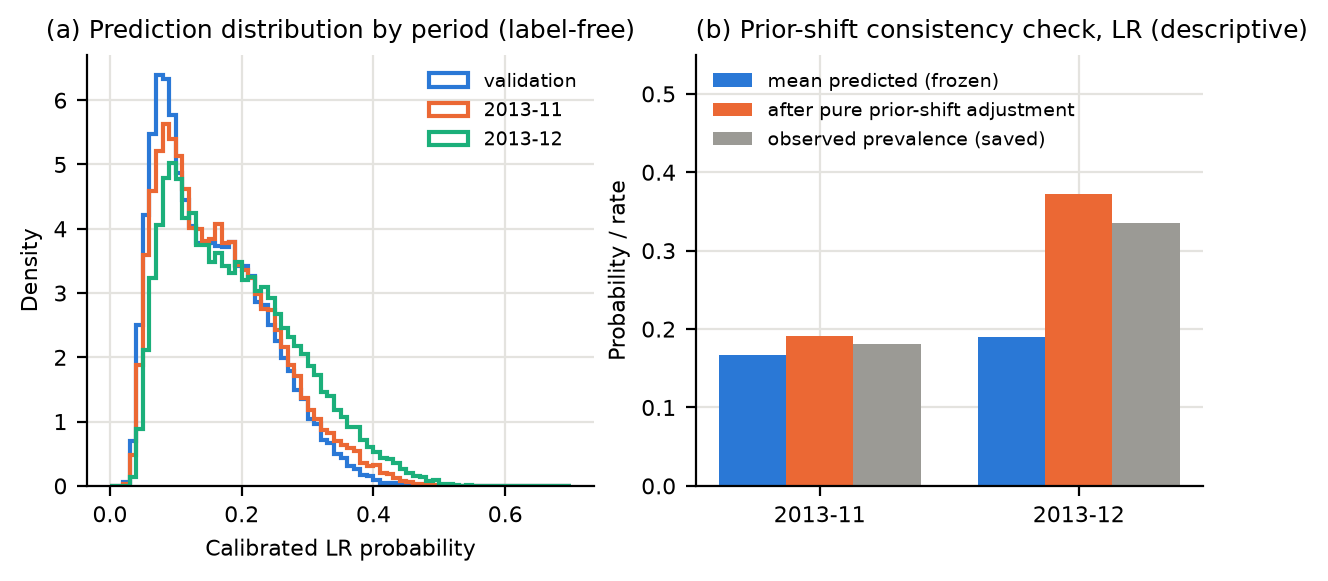
\includegraphics[width=0.8\linewidth]{stage9_prior_shift.png}
\caption{(a) Distribution of calibrated LR predictions by period (label-free). (b) Prior-shift
consistency check (descriptive; never applied).}
\label{fig:priorshift}
\end{figure*}

% =====================================================================
\section{Limitations and Threats to Validity}\label{sec:limitations}
\begin{itemize}
\item \textbf{Scope.} One year of departures from three New York airports. Seasonal effects cannot
be separated from events specific to 2013, and results may not generalise to other airports or years.
\item \textbf{Information.} No weather, same-day operational state, aircraft rotation or holiday
calendar was used. These limit what a day-ahead model can achieve.
\item \textbf{Population.} Cancelled and diverted flights are excluded, and their share varies by
carrier and month. Results apply to flights that operated and were recorded.
\item \textbf{Optimistic validation.} The validation months were reused for model selection, early
stopping, calibration choice and threshold selection.
\item \textbf{Calibration under shift.} Calibration was fitted on the calmest months of the year and
transferred poorly to a high-delay December. The cross-fitting procedure also reorders some flights
between months.
\item \textbf{Prior exposure.} Aggregate delay rates of the test months were seen during the data
audit, before the split was fixed. No test predictions or metrics existed before the single
evaluation, and the calibration and threshold rules were fixed beforehand.
\item \textbf{Training boundary.} The model is fitted on labels up to the last training day, which
a deployed model predicting the first validation day could not yet have. This affects one
validation day and no test day.
\item \textbf{Retrospective design.} The test period is a historical holdout, not a prospective
deployment, and the test-label lock is a procedural safeguard rather than access control.
\item \textbf{Interpretation.} Coefficients and importances describe associations, not causes. The
literature review is small and non-systematic.
\end{itemize}

% =====================================================================
\section{Conclusion and Future Work}\label{sec:conclusion}
Under a strict day-ahead information contract with verified leakage controls, a regularised
Logistic Regression ranked test flights by delay risk better than chance, better than XGBoost and
better than a constant base-rate forecast. Discrimination was modest, however (ROC AUC
\TestROCLR{}). The model did not provide probabilities more accurate than the base rate, and it
under-predicted in a high-delay December. No operating point met the targeted \MinPrecision{}
precision. A strictly day-ahead model built on schedule information and lagged history can
therefore offer coarse risk ranking, but not reliable individual delay alarms.

Future work, each item requiring a new and separately reported evaluation, includes:
\begin{itemize}
\item temporal deep-learning models (Phase~2; cf.~\cite{kim2016});
\item approved additional information sources, such as weather forecasts that are genuinely
available a day ahead;
\item recalibration strategies that can adapt to base-rate shift without using future labels;
\item evaluation across several years and airports.
\end{itemize}

\bibliographystyle{IEEEtran}
\bibliography{references}

\end{document}
